\section{Deterministic Sources}
A model for the deterministic (periodic) sources can be done using a staircase curve and an affine model. These two give upper bound for the arrival packets to the networks and can be used to design based on worst-case scenario.

The staircase arrival model is given by
\begin{flalign}
  R(t) \leq Sc(t) &= \left\lceil \frac{t - \mathrm{offset}}{T} \right\rceil \times P \ \ ,
\end{flalign}
%
where $R(t)$ is the real number of packets that have already arrived, $Sc(t)$ is the staircase model arrival curve, $\mathrm{offset}$ is the time offset measured from $t = 0$ to first packet arrival, $T$ is the period between packet arrivals and $P$ is the packet size.

The worst case happens when the offset goes to zero, this means, that the first packet arrives at time zero.
\begin{figure}[H]
  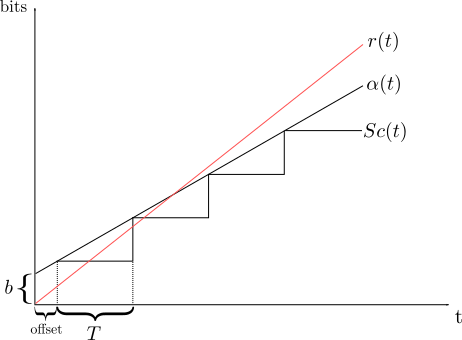
\includegraphics[width = .4\textwidth]{arrivalCurves}
  \caption{$Sc(t)$ is the staircase arrival curve, $\alpha(t)$ is the affine model arrival curve and $r(t)$ is the service curve defined by the capabilities of the CAN Bus.}
  \label{fig:arrivalCurves}
\end{figure}

The affine arrival model is given by
\begin{flalign}
  R(t) \leq \alpha (t) &= b + \frac{P}{T} t 
\end{flalign}
%
where $\alpha$ is the affine model arrival curve and $b$ is the crossing of the affine curve with the y-axis.

The relation between both models and the real arrival number of packets that have arrived is then given by
\begin{flalign}
  R &\leq Sc \leq \alpha 
\end{flalign}

\subsection{Wheels}
The staircase arrival model for each of the wheel sensors is
\begin{flalign}
  Sc_\mathrm{w} (t) &= \left\lceil \frac{t - \cancelto{0}{\mathrm{offset}} \ \ \ }{T_\mathrm{w}} \right\rceil \times P_\mathrm{w} \\
  Sc_\mathrm{w} (t) &= \left\lceil \frac{t}{0.04} \right\rceil \times 160, \ \ 
\end{flalign}
where $P_\mathrm{w} = 20\times 8 = 160$ since the packet size is \SI{20}{B}, which means that \SI{160}{b} arrive at each time interval, $T = 0.04$. The time offset is set to zero in order to model for worst case.
%
%\begin{where}
%  \va{Sc_\mathrm{w} (t)}{is the staircase model arrival curve for the wheel sensor data.}{}
%  \va{t}{is the time.}{}
%  \va{\mathrm{offset}}{is the time offset measured from $t = 0$ to first packet arrival.}{}
%  \va{T_\mathrm{w}}{is the period time for packet arrivals from the wheel sensors.}{}
%  \va{P_\mathrm{w}}{is the packet size containing the wheel sensor data.}{}
%\end{where}
%
%
The affine arrival model for each wheel sensor data is
\begin{flalign}
  \alpha_\mathrm{w} (t) &= b + \frac{P_\mathrm{w}}{T_\mathrm{w}} t  \\
  \alpha_\mathrm{w} (t) &= 160 + \frac{160}{0.04} t  = 160 + 6.4 t \ \ ,
\end{flalign}
where $b = P_\mathrm{w} = 160$ since the time offset is set to zero to model worst case.
%
%\begin{where}
%  \va{\alpha_\mathrm{w} (t)}{is the affine model arrival curve for the wheel sensor data}{}
%  \va{b}{is the crossing of the affine curve with the y-axis}{}
%\end{where}
%
%

\subsection{Electronic Speed Control (ESC)}
The staircase arrival model for the wheel sensor data is
\begin{flalign}
  Sc_\mathrm{ESC} (t) &= \left\lceil \frac{t - \cancelto{0}{\mathrm{offset}} \ \ \ }{T_\mathrm{ESC}} \right\rceil \times P_\mathrm{ESC} \\
  Sc_\mathrm{ESC} (t) &= \left\lceil \frac{t}{0.4} \right\rceil \times 64 \ \ ,
\end{flalign}
where $P_\mathrm{ESC} = 8\times 8=64$ since the packet size is \SI{8}{B}, which means that \SI{64}{b} arrive at each time interval, $T = 0.4$. The time offset is again set to zero in order to model for worst case.

The affine arrival model for the wheel sensor data is
\begin{flalign}
  \alpha_\mathrm{ESC} (t) &= b + \frac{P_\mathrm{ESC}}{T_\mathrm{ESC}} t  \\
  \alpha_\mathrm{ESC} (t) &= 64 + \frac{64}{0.4} t = 64 + 25.6 t \ \ ,
\end{flalign}
where $b = P_\mathrm{ESC} = 64$ since the time offset is set to zero to model worst case.

\subsection{Models encoded in RTC}
The stair case and the affine curves can be seen in \autoref{fig:ArrivalCurvesWheels} and \ref{fig:ArrivalCurvesESC}, as well as the service curve, which in this case is given by a 1MbpS CAN bus. 
\begin{figure}[H]
	\captionbox
	{
		Arrival curves for the four wheels and service curve for the CAN-bus.
		\label{fig:ArrivalCurvesWheels}
	}
	{
		\includegraphics[width=.46\textwidth]{figures/ArrivalCurvesWheels}
	}
	\hspace{5pt}
	\captionbox
	{
		Arrival curves for the ESC and service curve for the CAN-bus.
		\label{fig:ArrivalCurvesESC}
	}
	{
		\includegraphics[width=.46\textwidth]{figures/ArrivalCurvesESC}
	}
\end{figure}